% ! TeX root = ../thesis-main.tex
%----------------------------------------------------------------------------------------
\chapter{Analysis}
\label{chap:analysis}
%----------------------------------------------------------------------------------------
This chapter defines the scope, requirements, and use cases of \this, as well as their analysis and prioritization.

\section{Requirement analysis} \label{chap:analysis->sec:requirement-analysis}

Since the very beginning, \this aimed to redesign ScaFi using Scala 3 to improve the quality of the code, including but not limited to readability, maintainability, and reusability.
%
This time, using the \ac{XC} as the theoretical foundation, through which the \ac{FC} constructs could be implemented.

The project started interviewing the stakeholders, which are the developers and researchers who use ScaFi, to understand their needs and expectations.

The \textit{key users} identified for the library are:
\begin{itemize}
    \item \textit{End users}, that is, the developers who will use the library to implement their aggregate programs;
    \item \textit{Library developers}, who will extend the library with new features, constructs, and syntax;
    \item \textit{Researchers}, who will experiment with the calculus foundations but would benefit from reusing existing libraries.
\end{itemize}

During the interviews, both functional and technical requirements emerged and were collected and given priorities based on further discussions and feedback from the stakeholders.

\paragraph{Functional requirements} are the features that the library must provide to the users. The following are the most relevant functional requirements identified:
\begin{enumerate}[label=\textbf{F.\arabic*}]
    \item Redesign and implement a new \ac{API} for the \texttt{core} package\cref{chap:analysis->sec:scafi-analysis};
    \item Redesign and implement the \texttt{tests} package with acceptance tests, easy to read and understand, and that can be used as examples;
    \item Use the \ac{XC} as the foundation of the (default) implementation of constructs, while still providing a \ac{FC} based API;
    \item Develop an \textit{Alchemist incarnation}\footnote{\url{https://github.com/AlchemistSimulator/Alchemist}}\cite{alchemist}, enabling \this programs to run on the well-tested and widely used Alchemist simulator;
    \item Develop a minimal, pure Scala 3 simulator to run tests and examples without the need for external dependencies;
    \item Provide a new API for the \texttt{core} package that allows developers to import arbitrary ScaFi libraries and constructs into their programs without conflicts, in a seamless way;
    \item Prefer keeping the original, abbreviated names for core constructs like \texttt{nbr} and \texttt{rep}, now that they are widely adopted and recognized by the community;
    \item Experiment with Scala 3 to achieve new, compile time features for ScaFi that can improve the quality of the code and the user experience.
\end{enumerate}

\paragraph{Technical requirements} are the constraints and guidelines that the library must follow to ensure the quality of the code and the user experience.
\begin{enumerate}[label=\textbf{T.\arabic*}]
    \item Use Scala 3 as the host language;
    \item Enable quality options on the Scala 3 compiler such as explicit nulls (\cref{chap:background->sec:scala3->subsec:explicit-nulls}) and multiversal equality (\cref{chap:background->sec:scala3->subsec:multiversal-equality});
    \item Use \ac{SBT} as build system;
    \item Cross-build the project for \textit{scala-js}\footnote{\url{https://www.scala-js.org}};
    \item Cross-build the project for \textit{scala-native}\footnote{\url{https://scala-native.org}};
    \item Lint the code with \textit{scalafix}\footnote{\url{https://scalacenter.github.io/scalafix}} and/or \textit{scalafmt}\footnote{\url{https://scalameta.org/scalafmt}};
    \item Avoid using third-party libraries for the \texttt{core} package dependencies.
\end{enumerate}

Then, the requirements were discussed and prioritized, following the \ac{MoSCoW} method,
resulting in the table in \cref{tab:requirements-prioritization}.

\begin{table}[ht]
\centering
\caption{Requirements prioritization.}
\label{tab:requirements-prioritization}
\begin{tabular}{|>{\hspace{0pt}}m{0.362\linewidth}|>{\hspace{0pt}}m{0.277\linewidth}|>{\hspace{0pt}}m{0.238\linewidth}|} 
    \hline
    \textbf{Requirement} & \textbf{MoSCoW} & \textbf{Priority}  \\ 
    \hline
    F.1          & must   & high      \\ 
    \hline
    F.2          & must   & high      \\ 
    \hline
    F.3          & must   & high      \\ 
    \hline
    F.4          & could  & low       \\ 
    \hline
    F.5          & must   & high      \\ 
    \hline
    F.6          & should & average   \\ 
    \hline
    F.7          & should & average   \\ 
    \hline
    F.8          & won't  & low       \\ 
    \hline
    T.1          & must   & high      \\ 
    \hline
    T.2          & should & high      \\ 
    \hline
    T.3          & must   & high      \\ 
    \hline
    T.4          & could  & low       \\ 
    \hline
    T.5          & could  & low       \\ 
    \hline
    T.6          & should & low       \\ 
    \hline
    T.7          & should & average   \\
    \hline
\end{tabular}
\end{table}

Finally, before starting with the design of the solution, given that the project is a redesign of an existing library, the requirements were compared with the existing ScaFi library to identify the differences and similarities.



\section{ScaFi} \label{chap:analysis->sec:scafi-analysis}

The ScaFi repository\footnote{\url{https://github.com/scafi/scafi}} is organized in modules as pictured in \cref{fig:scafi-project-org}.
%
For most of the use cases, only a small subset of the modules should be imported.
%
The \this project is scoped around redesigning and implementing mainly the \texttt{core} package, implicitly including \texttt{commons}, and then the \texttt{simulator} and \texttt{tests} packages, albeit with a minimal version of the simulator in pure Scala 3.
%
The rest of the modules, providing various \ac{GUI} implementations, demos, as well as integration with \textit{Akka}\footnote{\url{https://akka.io}} for actual deployment of real-world aggregate applications, are out of the scope of \this, and are addressed in \cref{chap:conclusion-and-future-work}.

\begin{figure}
    \centering
    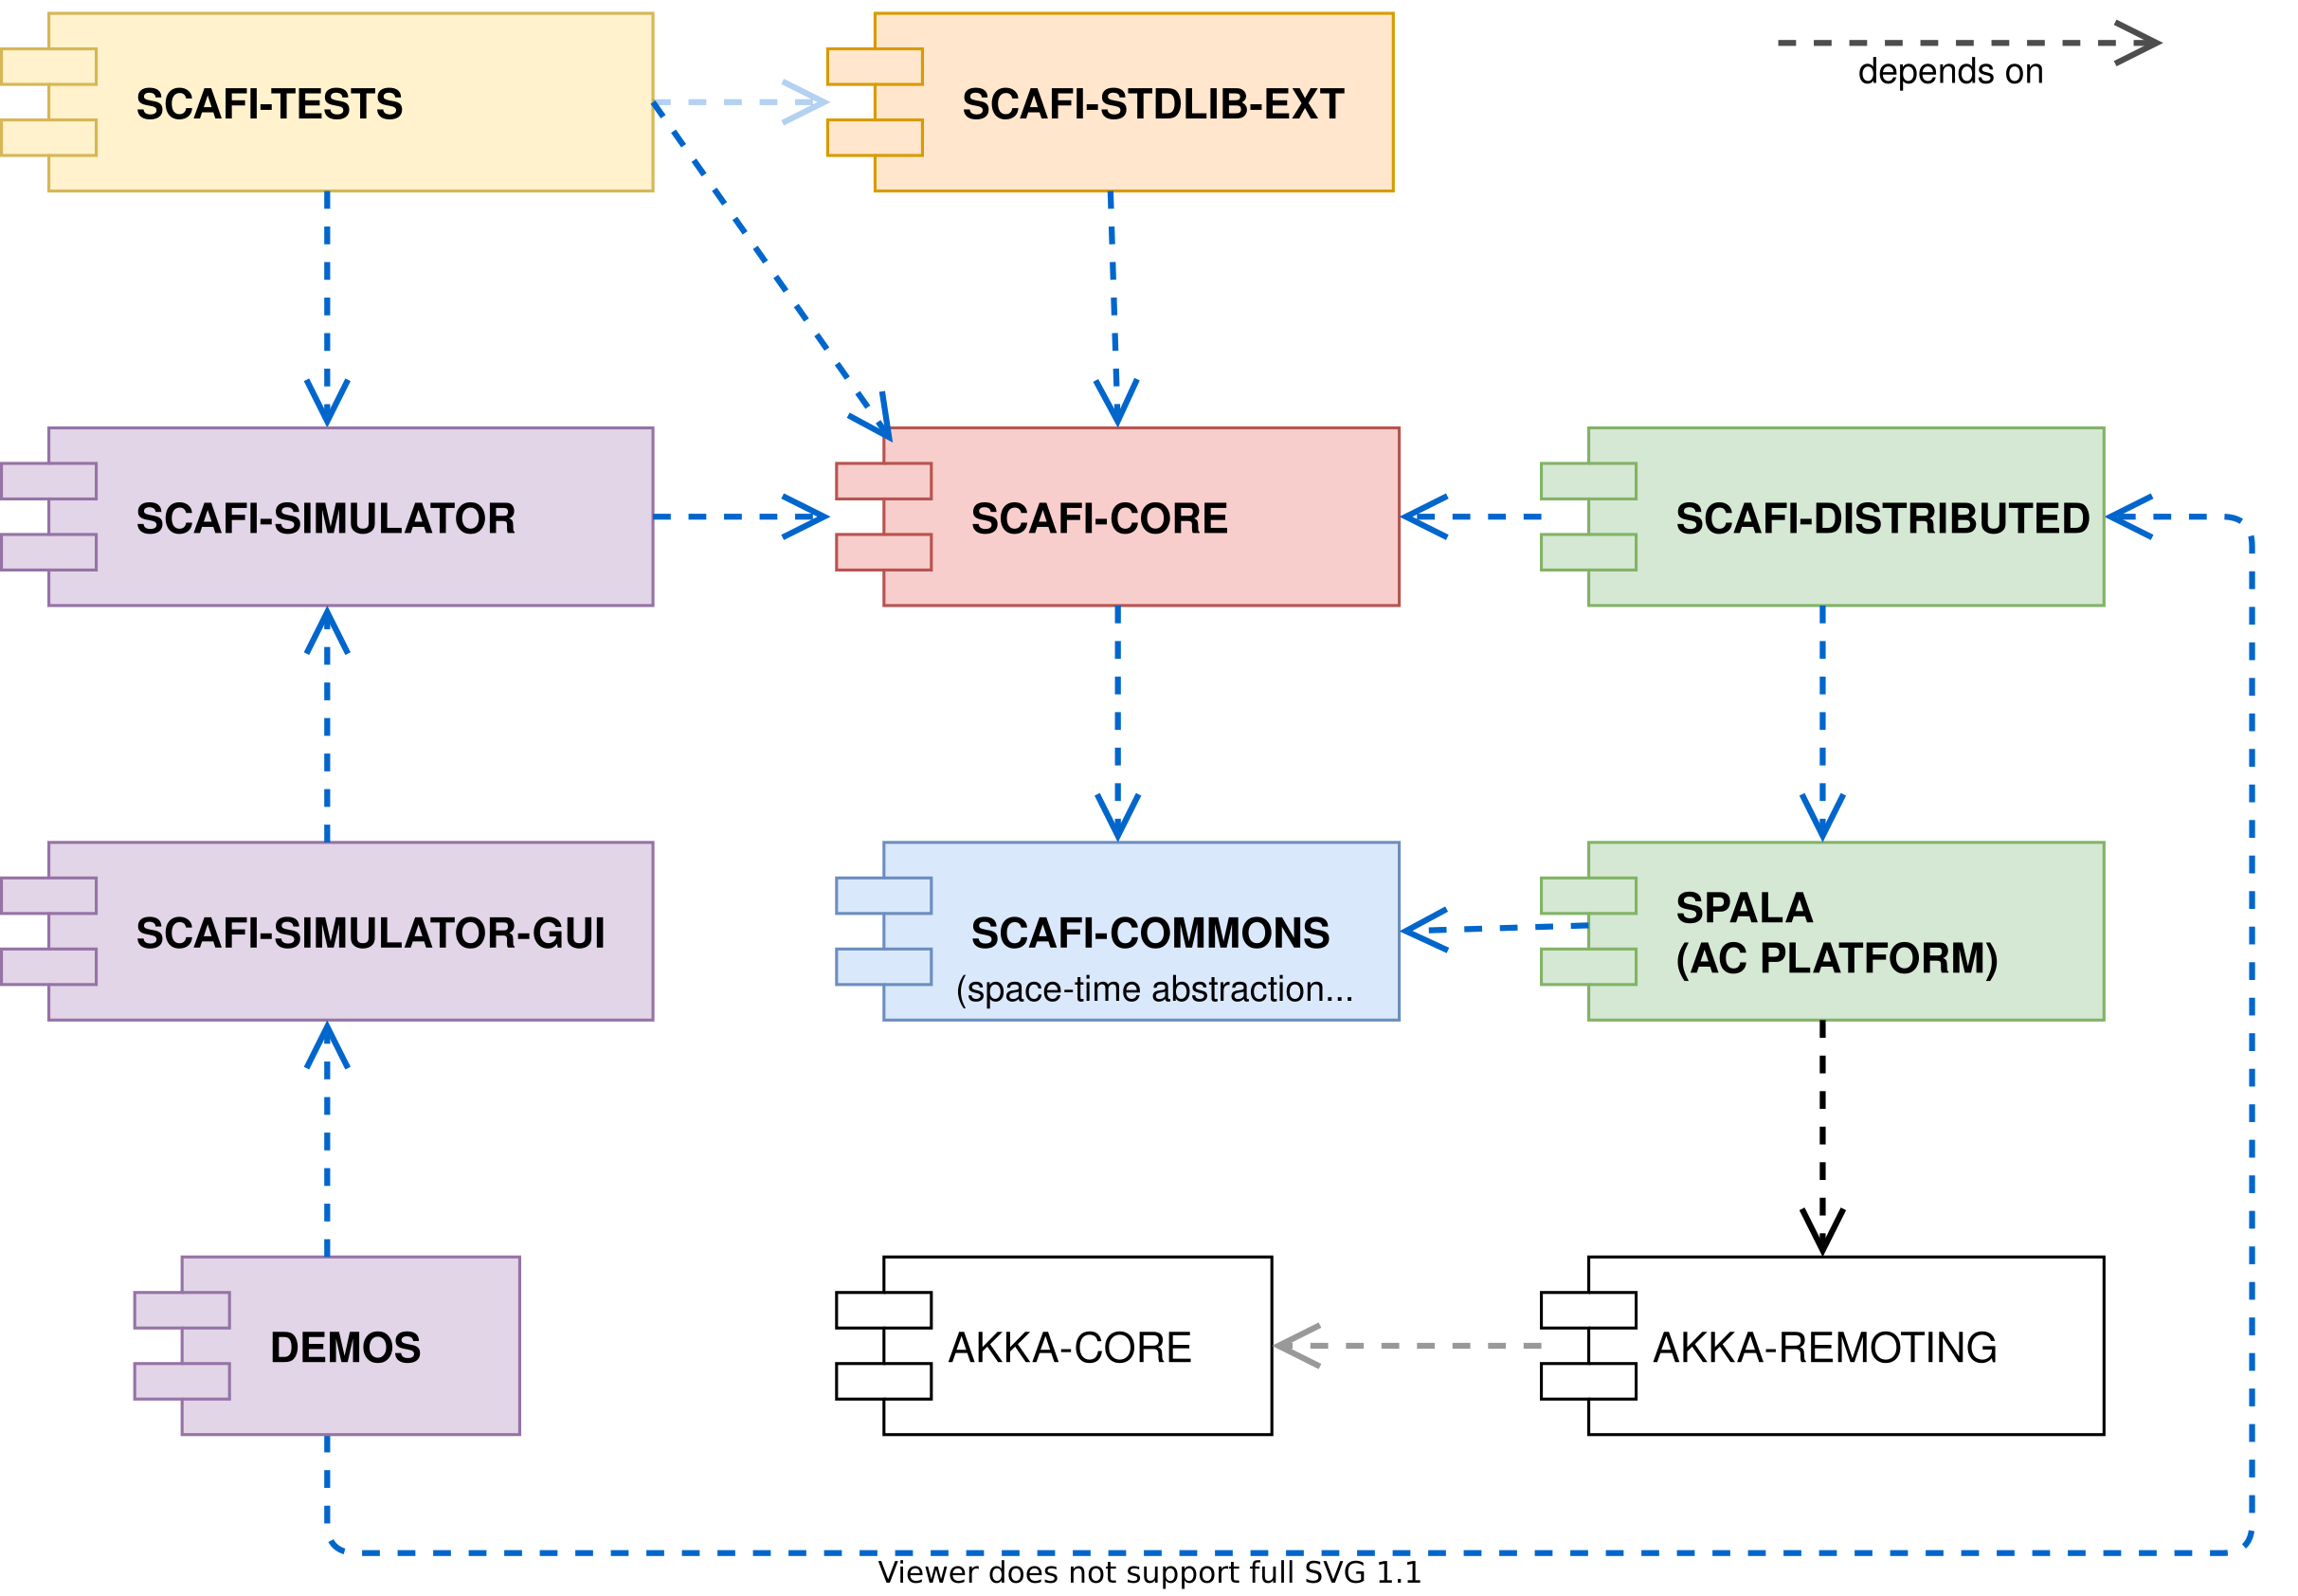
\includegraphics[width=.8\linewidth]{figures/scafi-project-org.drawio.png}
    \caption{ScaFi project organization.}
    \label{fig:scafi-project-org}
\end{figure}

Inside the \texttt{core} package of the \texttt{core} module, a \texttt{Core} trait serves as the root of the family of traits, defining a set of abstract type members and traits, such as \texttt{Context}, that represents the context of the aggregate program execution.
%
A trait \texttt{Language} defines a \texttt{Constructs} trait with the core syntax of \ac{FC}, such as \texttt{rep}, \texttt{nbr}, and \texttt{foldhood}, plus additional utilities such as \texttt{mid(): ID} for retrieving the device own id and \texttt{sense[A](name: CNAME): A} for sensing a value from the environment.
%
The \texttt{RichLanguage} trait extends \texttt{Language} with additional constructs, such as \texttt{branch}, \texttt{foldhoodPlus}, and \texttt{maxHood}.
%
Finally, the \texttt{Semantics} trait implements the \ac{FC} constructs, the value tree building, and the foldhood context semantics, further detailed in \cref{chap:analysis->sec:scafi-analysis->subsec:foldhood-semantics}.
%
In addition to that, the \texttt{core} module contains other packages, such as \texttt{lib} with standard libraries, and the utilities to provide a fully-fledged aggregate program execution environment called \textit{incarnation}.
%
The \texttt{distributed} and \texttt{spala} modules enable ScaFi to run on real-world distributed applications by leveraging integration with the \textit{Akka framework}\footnote{\url{https://akka.io}} and with other supportive libraries such as \textit{Java Swing} and the \textit{Play Framework}\footnote{\url{https://www.playframework.com}}.
%
Finally, the \texttt{simulator} and affiliated modules provide an advanced simulation suite featuring spacial and temporal simulation and multiple \ac{GUI} options, including a tridimensional renderer.

To use a library component in ScaFi, the user must mix in the library trait with the \texttt{AggregateProgram} base class, as shown in \cref{lst:using-libraries-in-scafi}.
%
As a consequence, all the transitive dependencies of the mixed-in libraries are visible in the scope of the program, so libraries must be written in a way that avoids conflicts with other libraries.

\lstinputlisting[float, language=Scala, caption={Using a library component in ScaFi.}, label={lst:using-libraries-in-scafi}]{listings/scafi-using-libraries.scala}

After defining a program as a method named \texttt{main} within the \texttt{AggregateProgram} extension, the user can run the program on the simulator through the \texttt{Launcher}, an extension to Scala's \texttt{App} that provides a \texttt{launch} method to start the simulation with one of the available \acp{GUI}.

\this aims to redesign and implement the \texttt{core} package in such a way that implementing a similarly advanced simulation suite would still be possible, while improving the quality of the code and the user experience.

\subsection{The foldhood semantics in ScaFi} \label{chap:analysis->sec:scafi-analysis->subsec:foldhood-semantics}

Using the concept of a stateful \quotes{virtual machine}, ScaFi tracks at its core the context of the evaluation of expressions inside the aggregate program.
%
It tracks nested invocations of core constructs, as well as the scope of the foldhood expressions, which are evaluated for every neighbor of the device, and the result of each evaluation is combined into a single value.
%
This design choice avoids the definition of an explicit type for fields, resulting in a clean syntax but leaving the awareness of the underlying field-like nature of the foldhood semantics to the user.
%
For instance, the fact that \texttt{nbr{nbr{x}}} does not make sense inside a foldhood is something that the user must be aware of, given that the compiler and the virtual machine do not enforce it.
